\subsection{Raumtypen}\label{raumtypen}

% include figure
\begin{figure}[ht]
    \centering
    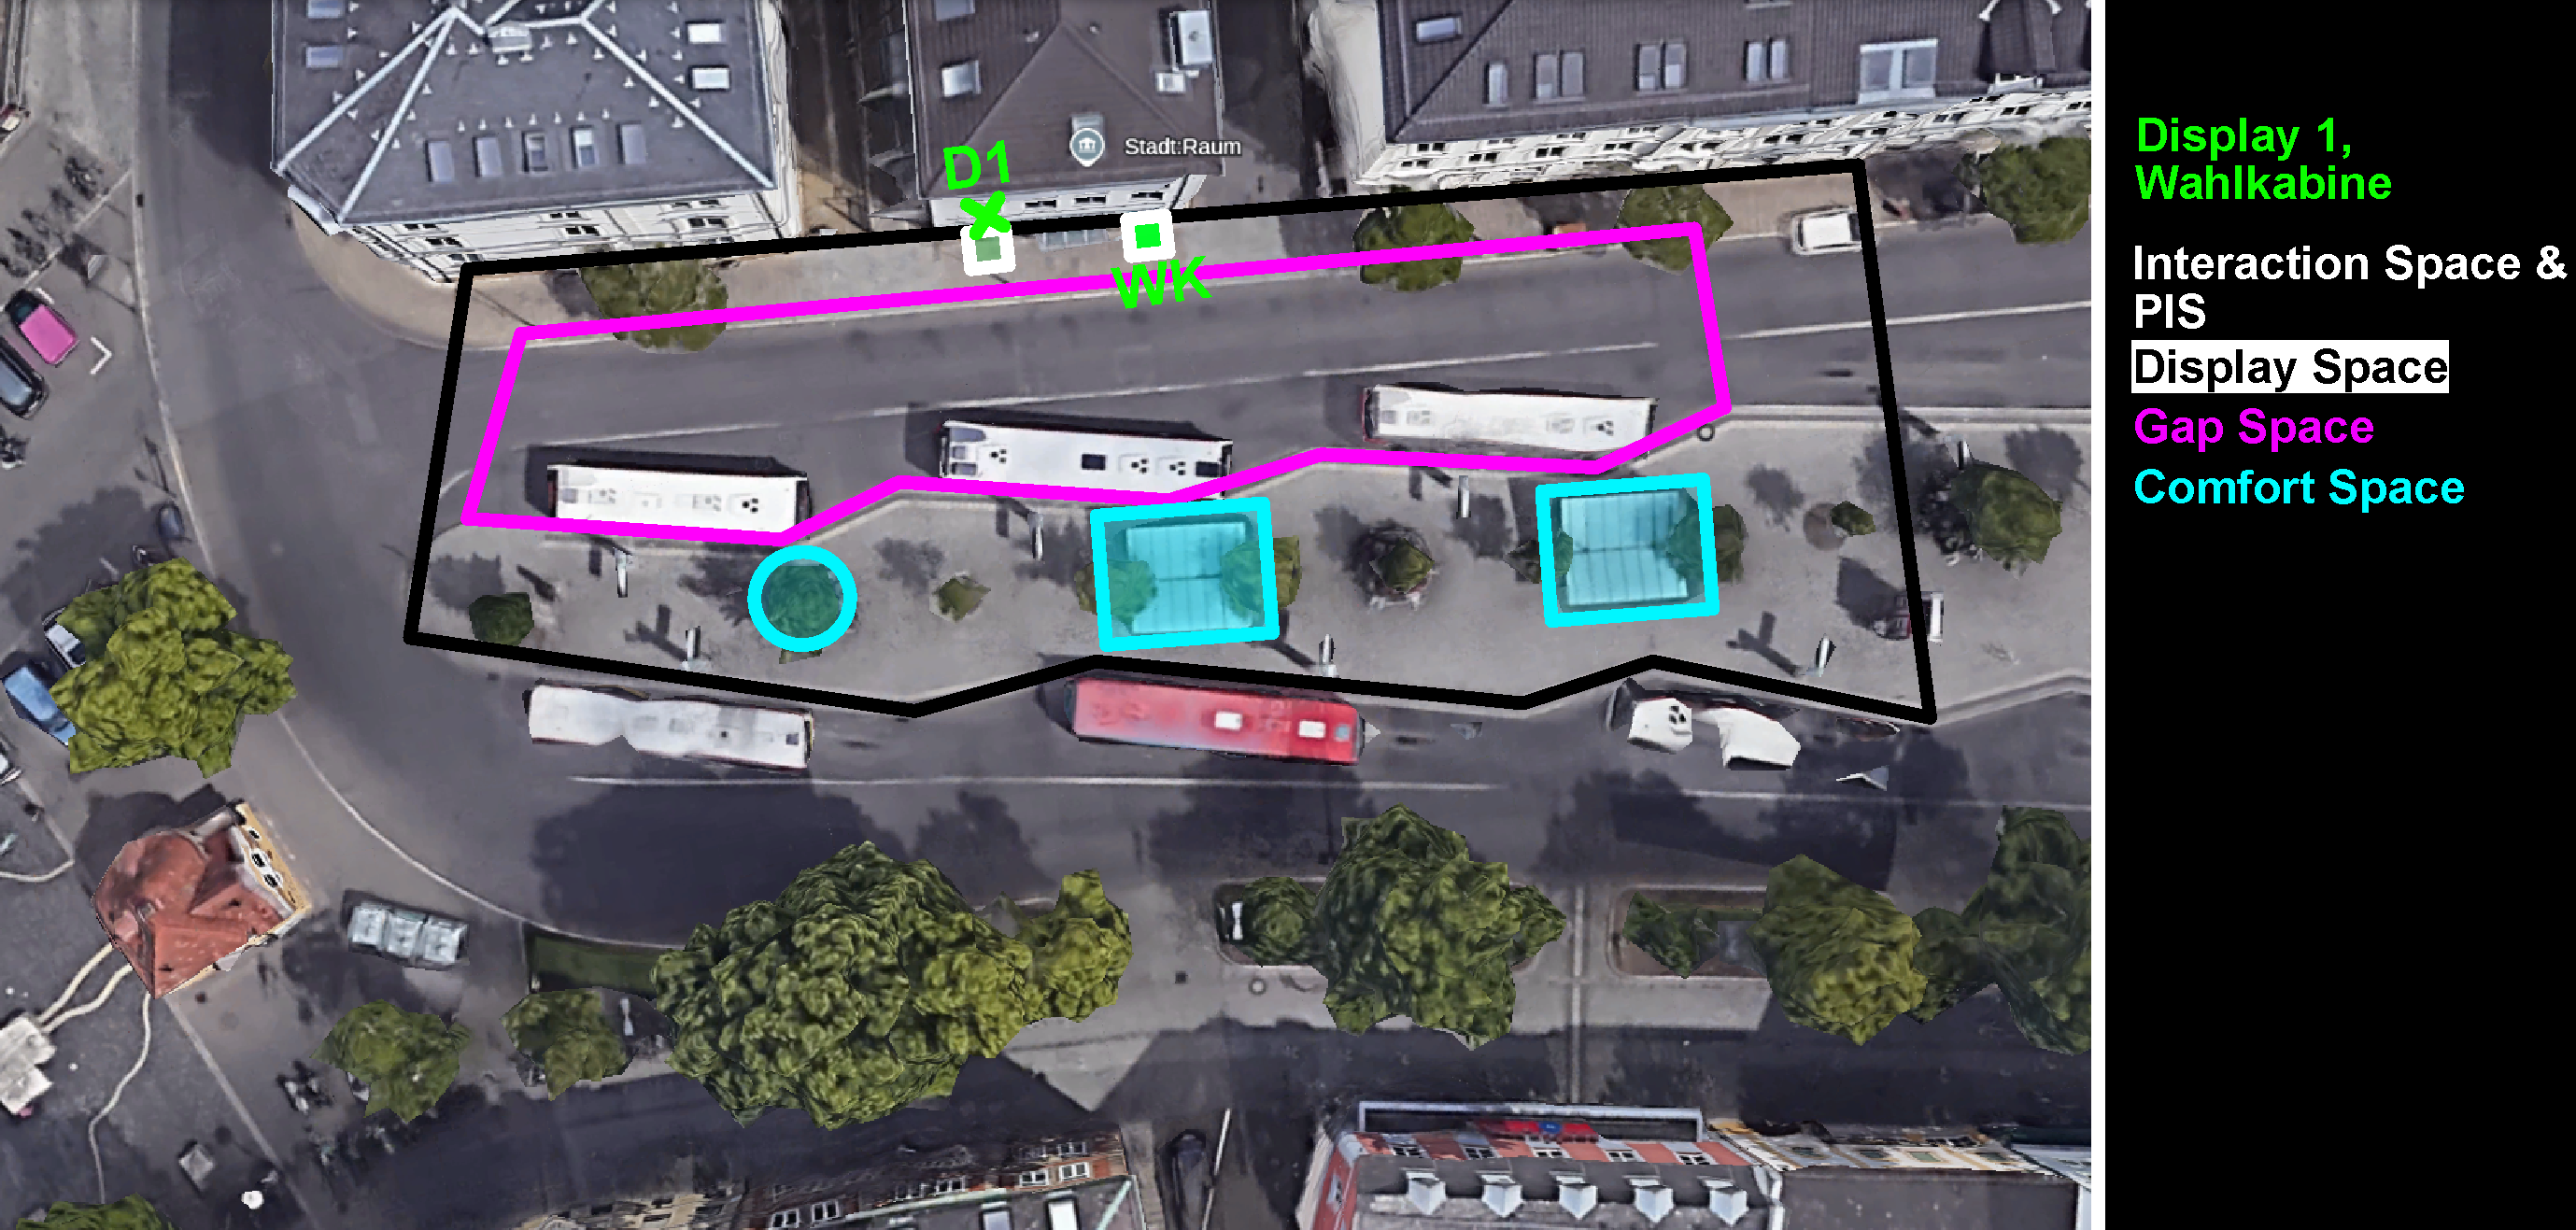
\includegraphics[width=0.8\textwidth]{figures/raumtypen.pdf}
    \caption{Raumtypen am Stadt:Raum}
    \label{fig:raumtypen}
\end{figure}

Im folgenden Kapitel werden die Raumtypen \cite{raumtypen} am Stadt:Raum beschrieben, die für die Installation relevant sind.

\subsubsection{Display Space}\label{display-space}

Im markierten Display Space sind nicht aus jeder Position beide Displays sichtbar, aus bestimmten Positionen ist sogar gar kein Display sichtbar.
Allerdings ist mindestens die Wahlkabine aus jeder Position sichtbar, weshalb wir den Display Space entsprechend groß gewählt haben.
Angrenzend an den Display Space befindet sich der Activation Space (nicht extra eingezeichnet), an dem Passanten auf die Installation aufmerksam werden /könnten/.

\subsubsection{Interaction Space}\label{interaction-space}

Der Interaction Space befand sich unmittelbar vor Display 1 und in der Wahlkabine.
Durch die Wahlkabine war der Interaction Space an dieser Stelle sehr isoliert, wohingegen der Interaction Space vor Display 1 auch Potential für Gruppeninteraktionen bot.
In der Praxis hat sich gezeigt, dass auch Gruppen aus zwei Personen gemeinsam vor Display 1 stehen blieben und über die Ergebnisse sprachen.

\subsubsection{Gap Space}\label{gap-space}

Aufgrund der Beschaffenheit des ZOB entstand durch die von Bussen befahrene Straße zwischen Gehsteig und Haltestellen ein toter Raum, der Distanz zur Installation schaffte.
Insbesondere wenn ein Bus für mehrere Minuten an einer Haltestelle stand und die Sicht auf die Installation verdeckte, war der Raum hinter dem Bus verloren.

\subsubsection{Comfort Space}\label{comfort-space}

Kurz hinter dem Gap Space befinden sich mehrere Sitzgelegenheiten an den Haltestellen, die Comfort Spaces bilden.
Von hier aus ist das Geschehen an der Installation beim Warten auf den Bus direkt beobachtbar.
Der mittlere Comfortspace ist der Interessanteste, da von hier aus sowohl die Wahlkabine als auch Display 1 eingesehen werden können.
Wir nahmen an, dass an dieser Stelle auch ein Social Interaction Space entstehen könnte, indem das Beobachtete in Gruppen zum Gesprächsthema wird und daraus neue Trigger zur Interaktion mit der Installation entstehen.
Dies konnten wir leider nicht beobachten.
Das Queren der Straße zum Abgeben der Stimme war der Ausnahmefall.